The theorem we will prove is that integrals over homotopic curves are equal. Admittedly this seems a bit strange but really is just a restatement of the fact that the integral of closed forms over the boundary of rectangles is 0. The key idea is that integrals over homotopic curves can be computed by working over the boundary of $[0, 1] \times [0, 1]$ since we can pullback via the homotopy. Then it is just a matter of looking at the consequence of this. This is all made more precise in \autoref{thm:integral-over-homotopic-curves}.

We also present a second proof of the same theorem for which we need the following lemma generalising the notion of primitives along curves.
\begin{lemma}
Let $\omega$ be a closed form in $\Omega$. Let $\gamma: [a, b] \times [c, d] \to \Omega$ be a continuous map. Then there is a continuous function $f: [a, b] \times [c, d] \to \C$ such that for every $(s_0, t_0) \in [a, b] \times [c, d]$ that there is a primitive $F$ of $\omega$ defined on a neighbourhood of $\gamma(s_0, t_0)$ such that
$$ f(s, t) = F(\gamma(s, t))$$
for all $(s, t)$ in a neighbourhood of $(s_0, t_0)$. Moreover, $f$ is unique up the addition of a constant.
\end{lemma}
\begin{proof}
    The proof of uniqueness is the exact same as before (see \autoref{prop:primitive-along-curve}). In particular, the difference of two different primitives along $\gamma$ is the difference of two genuine primitives of $\omega$ in a neighbourhood. So the difference is locally constant but since the domain is connected it must be constant everywhere. 
    
    The proof of existence will be quite similar to the previous proposition as well. First we choose partitions $\{s_i\}$ and $\{t_j\}$ of $[a, b]$ and $[c, d]$ respectively so that $\gamma([s_{i - 1}, s_i] \times [t_{j - 1}, t_j])$ is contained in an open disk $U_{ij}$ in which $\omega$ has a primitive $F_{ij}$.
    
    Suppose we fix a $j$. Then two primitives $F_{i, j}$ and $F_{i + 1, j}$ defined on $U_{ij}$ and $U_{i + 1, j}$ respectively differ by a constant in the intersection of the two disks. Thus we can adjust the constants to ensure that they agree on $\bigcup_i [s_{i - 1}, s_i] \times [t_{j - 1}, t_j]$. Doing this for all $j$, we find primitives $f_j$ along $\gamma|_{[a, b] \times [t_{j - 1}, t_j]}$ by defining $f_j = F_{i, j} \circ \gamma$ in $[s_{i -1}, s_i] \times [t_{j - 1}, t_j]$. The functions $f_j$ and $f_{j + 1}$ may be different on the curve $[a, b]  \times \{t_j\}$ but they are primitives along a curve so once again they only differ by a constant. Thus we can adjust the constants to define $f$ on all of $[a, b] \times [c, d]$.
\end{proof}

\begin{theorem}\label{thm:integral-over-homotopic-curves}
Let $\omega$ be a closed form in an open set $\Omega \subset \C$. Let $\gamma_0, \gamma_1: [0, 1] \to \C$ be homotopic, continuous curves (they might be homotopic with fixed endpoints or homotopic as closed curves). Then
$$ \int_{\gamma_0} \omega = \int_{\gamma_1} \omega $$
\end{theorem}
\begin{proof}
    Suppose $\gamma_0, \gamma_1$ are homotopic with fixed endpoints. Let $\gamma: [0, 1] \times [0, 1] \to \Omega$ be the homotopy between them. This means that $\gamma(0, t) = \gamma_0(t), \gamma(1, t) = \gamma_1(t)$ and $\gamma(s, 0) = \gamma_0(0) = \gamma_1(0)$ and $\gamma(s, 1) = \gamma_0(1) = \gamma_1(1)$. 
    
    First we observe that
    \begin{align*}
        \int_{\gamma(\partial I^2)} \omega = \int_{\partial I^2} \gamma^*\omega = 0
    \end{align*}
    since $\gamma^*\omega$ is closed (one way of seeing this is to note that $d(\gamma^*\omega) = \gamma^*(d \omega) = 0$).

    On other hand let us compute what this integral is without pulling back. Let $\sigma_1, \sigma_2, \sigma_3, \sigma_4$ denote the bottom, right, top, and left edge of $[0, 1] \times [0, 1]$ all oriented as the boundary of the square. Then we see that
    \begin{align*}
        \int_{\gamma(\partial I^2)} \omega &= \int_{\gamma(\sigma_1 + \sigma_2 + \sigma_3 + \sigma_4)} \omega = \int_{\gamma(\sigma_1)} \omega + \int_{\gamma(\sigma_2)} \omega + \int_{\gamma(\sigma_3)} \omega + \int_{\gamma(\sigma_4)} \omega
    \end{align*}
    Since $\gamma$ is a homotopy (between curves with fixed endpoints) we know $\gamma(\sigma_1)$ and $\gamma(\sigma_3)$ are constant while $\gamma(\sigma_2) = \gamma_1$ and $\gamma(\sigma_4) = -\gamma_0$. Thus we get
    $$\int_{\gamma_1} \omega - \int_{\gamma_0} \omega = 0$$

    For closed curves we would find that the integral over $\sigma_1$ and $\sigma_3$ cancel out leading us to the same conclusion.
\end{proof}
\begin{proof}
    Suppose $\gamma_0, \gamma_1$ are homotopic with fixed endpoints. Let $\gamma: [0, 1] \times [0, 1] \to \Omega$ be the homotopy between them. This means that $\gamma(0, t) = \gamma_0(t), \gamma(1, t) = \gamma_1(t)$ and $\gamma(s, 0) = \gamma_0(0) = \gamma_1(0)$ and $\gamma(s, 1) = \gamma_0(1) = \gamma_1(1)$. 
    
    Let $f$ be a primitive of $\omega$ along $\gamma$. Note that $f(s, 0)$ and $f(s, 1)$ is constant as we vary $s$. This is because locally $f = F \circ \gamma$ where $F$ is some local primitive of $\omega$. But we know $\gamma$ is constant as we vary the first component, given that the second component is 0 or 1. In particular this means that $f(0, 0) = f(1, 0)$ and $f(0, 1) = f(1, 1)$. Thus we find
    $$ \int_{\gamma_0} \omega = f(0, 1) - f(0, 0) = f(1, 1) - f(1, 0) = \int_{\gamma_1} \omega $$
    where we use the fact that $f(0, t)$ and $f(1, t)$ are primitives along $\gamma_0$ and $\gamma_1$ respectively.

    The result for closed curves can actually be deduced from the above case. Let $\gamma_0$ and $\gamma_1$ be two homotopic closed curves. Let $\gamma$ be the homotopy between them. Let $\sigma(t)$ denote the path $\gamma(t, 0)$ which connects $\gamma_0(0)$ and $\gamma_1(0)$. Then $\gamma_0 * \sigma$ is also a path from $\gamma_0(0)$ to $\gamma_1(0)$ while $\sigma * \gamma_1$ is another such path. These two paths are obviously homotopic (the homotopy is given by following $\sigma$ until time $s$, then following $\gamma(s,-)$, and then following $\sigma$ until the end, see \autoref{fig:closed-curve-homotopy}). Thus the integral over the two paths is the same. Both paths have the integral over $\sigma$ which we can then cancel allowing us to conclude that the integral over the closed curves is equal.

    \begin{figure}
        \centering
        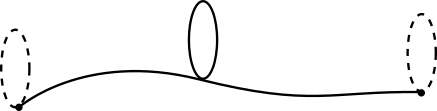
\includegraphics{Images/closed_curve_homotopy.png}
        \caption{Homotopy given by $\sigma$ until time $s$, followed by $\gamma(s,-)$, followed by $\sigma$ until the end}
        \label{fig:closed-curve-homotopy}
    \end{figure}
\end{proof}
\begin{corollary}
    In a simply connected open set every closed form has a primitive.
\end{corollary}
\begin{proof}
    Recall that a simply connected set is one that is connected and where every closed curve is homotopic to a point. Furthermore, a form has a primitive if and only if the integral over every closed curve is 0 (see \autoref{prop:exact-equivalence}). Hence we will show that the integral over any closed curve is 0. 
    
    Let $\gamma$ be a closed curve in the simply connected open set. We know $\gamma$ is homotopic to a constant curve and by the previous theorem we know that integral over homotopic curves are equal. Moreover, the integral over a constant curve is necessarily 0 (we are effectively integrating over a point, or to put it more precisely the `path' is constant so when we compute the pullback it becomes 0). Therefore the integral over $\gamma$ is 0 as desired. 
\end{proof}

Some examples of simply connected open sets are disks and rectangles. A slightly less familiar example (which in fact includes the previous two) is a star-shaped open set. A star shaped set is a set $S$ which contains a point $a$ so that for any point $x$ in $S$ the line connecting $a$ and $x$ is also contained in $S$. In this case it is clear that any closed curve $\gamma_0$ in $S$ is homotopic to the point $a$. In fact, we can even explicitly give the homotopy $\gamma(s, t) = (1 - s)a + s\gamma_0(t)$.

This also means we can define a branch of $\log z$ in any simply connected set not containing 0 by
$$ \log z = w_0 + \int_{z_0}^z \frac{dz}{z} $$
where $z_0$ is some fixed point in the set and $w_0$ is such that $e^{w_0} = z_0$ (to be fair, the above is improper notation since the bounds of the integral may be complex. What we mean of course by the integral is to choose a path from $z_0$ to $z$ and to integrate over that. We know the choice of path is irrelevant which justifies the notation). 

We can also use this to conclude that $\C \setminus \{0\}$ is not simply connected since 
$$ \int_{S^1} \frac{dz}{z} = 2\pi i \neq 0 $$

\subsection{Cauchy's Integral Formula}
Cauchy's integral formula allows us to compute the value of a holomorphic function at a point by integrating along the boundary of a region containing that point. This relationship between evaluating the function and integrating it is exactly what we need in order to show that holomorphic functions are analytic.
\begin{definition}[Winding Number]
Let $\gamma$ be a closed curve in an open set $\Omega$ and let $a \in \Omega$ be a point lying outside the curve. Then the winding number of $\gamma$ with respect to $a$ is given by
$$ w(\gamma, a) = \frac{1}{2\pi i} \int_\gamma \frac{1}{z - a}dz $$
Note that $w(\gamma, a)$ is always an integer.
\end{definition}

As the name suggests, the winding number counts the number of times that the curve winds around the point $a$. Thus for example $w(e^{2\pi it}, 0) = 1$ while $w(e^{4\pi it}, 0) = 2$.The winding number has some very nice properties. 
\begin{enumerate}
    \item Fix some $a$. Then $w(\gamma, a)$ is invariant under homotopies of $\gamma$ that do not pass through $a$. This follows from \autoref{thm:integral-over-homotopic-curves}. 
    \item In particular, if $\gamma$ lies in a simply connected open set not containing $a$ then $w(\gamma, a) = 0$. This follows from the same theorem since we can create a homotopy to a point.
    \item Fix the curve $\gamma$. Then $w(\gamma, a)$ is constant on connected components of the complement of $\gamma$. In order to prove this, it suffices to show that $w(\gamma, -)$ is locally constant. Note that shifting $a$ so that it remains in the same connected component is the same as shifting $\gamma$ (via a homotopy not passing through $a$). Thus by the first point, we know $w(\gamma, -)$ is locally constant.
    \item A specific but useful case of the previous point is the following,  $\gamma$ is a circle described in the positive sense (i.e. $w(\gamma, center) = 1$) then $w(\gamma, a) = 1$ if $a$ is inside the circle and 0 otherwise.
\end{enumerate}
With the winding number in hand, we can compute certain integrals very easily.
\begin{theorem}[Cauchy's Integral Formula]
Let $\Omega$ be an open subset of $\C$ and let $f$ be a holomorphic function on $\Omega$. Let $\gamma$ be a nullhomotopic closed curve in $\Omega$ and let $a$ be a point in $\Omega$ that is not on $\gamma$. Then
$$ \frac{1}{2\pi i} \int_{\gamma} \frac{f(z)}{z - a}dz = w(\gamma, a) \cdot f(a) $$
\end{theorem}
\begin{proof}
    We define
    \begin{align*}
        g(z) = \begin{cases}
        \frac{f(z) - f(a)}{z - a} &\text{ if } z \neq a\\
        f'(a) &\text{ if } z = a
        \end{cases}
    \end{align*}
    Note that $g$ is continuous on $\Omega$ and holomorphic on $\Omega \setminus \{a\}$. Then we know that $g(z) dz$ is closed by Cauchy's Theorem (see \autoref{cor:cauchy-thm-general}). Therefore
    $$ 0 = \int_\gamma g(z) dz = \int_{\gamma} \frac{f(z) - f(a)}{z - a} dz $$
    where for the first equality we use the fact that $\gamma$ is nullhomotopic. Thus we conclude that
    $$ \int_{\gamma} \frac{f(z)}{z - a}dz = \int_\gamma \frac{f(a)}{z - a}dz = 2\pi i f(a) w(\gamma, a) $$
\end{proof}
\begin{corollary}
    If $f(z)$ is holomorphic in the neighbourhood of a closed disk $D$ and $\gamma$ is the boundary of $D$ (in the positive sense) then
    \begin{align*}
        \frac{1}{2\pi i} \int_\gamma \frac{f(z)}{z - a}dz =
        \begin{cases}
            f(a) &\text{ if $a$ is inside the circle}\\
            0 &\text{ if $a$ is outside the circle}
        \end{cases}
    \end{align*}
\end{corollary}
\begin{proof}
    This follows from the previous lemma by noting that $w(\gamma, a)$ is 1 if $a$ is inside the circle and $0$ if it's outside.
\end{proof}
A consequence of Cauchy's Integral Formula is that holomorphic functions are in fact infinitely differentiable. For example suppose $f$ is holomorphic in an open disk $D$. Let $\gamma$ be the boundary of some circle just slightly smaller than $D$. Then for any $z$ inside this smaller circle, we know by the corollary above that
$$ f(z) = \frac{1}{2\pi i} \int_{\gamma} \frac{f(\zeta)}{\zeta - z} d\zeta $$
But this means that
$$ f'(z) = \frac{1}{2\pi i} \int_\gamma \frac{f(\zeta)}{(\zeta - z)^2} d\zeta $$
and more generally
$$ f^{(n)}(z) = \frac{n!}{2\pi i} \int_\gamma \frac{f(\zeta)}{(\zeta - z)^{n + 1}} d\zeta $$


Let us summarise everything we have learned so far.
\begin{proposition}
Suppose $f$ is a continuous function in the open set $\Omega$. Then the following are equivalent:
\begin{enumerate}
    \item $f$ is holomorphic in $\Omega$
    \item $f(z) dz$ is closed
    \item Given a closed disk $D$ in $\Omega$ and $\gamma$ its oriented boundary, we have
    $$ f(z) = \frac{1}{2\pi i} \int_{\gamma} \frac{f(\zeta)}{\zeta - z} d\zeta $$
    for every $z$ in the interior of $D$.
\end{enumerate}
\end{proposition}
\begin{proof}
    We know that $(1) \Rightarrow (2)$ is simply Cauchy's theorem (see \autoref{thm:cauchy-thm}) and $(1) \Rightarrow (3)$ is exactly Cauchy's Integral formula. We just checked $(3) \Rightarrow (1)$ above since you can swap the integration and differentiation which is what gave us all the derivatives of $f$. Thus we only need to show $(2) \Rightarrow (1)$ to finish the proof. That particular statement is sometimes called Morera's Theorem.
    
    Since $f(z) dz$ is closed, we know it locally has a primitive, $g(z)$. Moreover, we know that $g$ is holomorphic. This means that $g'(z) = f(z)$ must also be holomorphic since the derivative of a holomorphic function is itself holomorphic.
    
\end{proof}
\begin{corollary}
    A continuous function which is holomorphic except on a line is holomorphic everywhere.
\end{corollary}
\begin{proof}
    Suppose $f(z)$ is a continuous function that is holomorphic everywhere except maybe on a line. Then we know by Cauchy's Theorem that $f(z)dz$ is closed but this means that $f(z)$ is holomorphic by the above.
\end{proof}

\subsection{Applications of Cauchy's Formula}
A very important fact that we can now show quite easily is that holomorphic functions always have a convergent power series expansion (at least locally), which is to say that being holomorphic and analytic are equivalent conditions in the complex setting.
\begin{theorem}
Suppose $f(z)$ is a holomorphic function in the disk $\abs{z} < R$. Then $f$ has a convergent power series expansion in this disk.
\end{theorem}
\begin{proof}
    Let $z$ be a point inside the disk and let $r$ be such that $\abs{z} < r < R$. Suppose $\zeta$ is such that $\abs{\zeta} = r$. Then
    $$ \frac{1}{\zeta - z} = \frac{1}{\zeta} \left(1 - \frac{z}{\zeta} \right)^{-1} = \frac{1}{\zeta} \left( 1 + \frac{z}{\zeta} + \frac{z^2}{\zeta^2} + \cdots \right) $$
    Then we can use this in Cauchy's Integral Formula to obtain the power series expansion for $f$.
    \begin{align*}
        f(z) &= \frac{1}{2\pi i} \int_{\gamma} \frac{f(\zeta)}{\zeta - z} d\zeta\\
        &= \frac{1}{2\pi i} \int_\gamma \sum_{n = 0}^\infty \frac{z^n f(z)}{\zeta^{n + 1}} d\zeta\\
        &= \sum_{n = 0}^\infty \left( \frac{1}{2\pi i} \int_\gamma \frac{f(\zeta)}{\zeta^{n + 1}} d\zeta \right) z^n
    \end{align*}
    We can swap the summation and integration because the convergence of the series is uniform (being a geometric series). 
    
    We know that the coeffecients $a_n$ in a Taylor expansion (centered at 0) are simply given by $\frac{f^{(n)}(0)}{n!}$. We have computed $f^{(n)}(z)$ previously and using this we would find the coefficients should be
    $$ a_n = \frac{f^{(n)}(0)}{n!} = \frac{1}{2\pi i} \int_\gamma \frac{f(\zeta)}{\zeta^{n + 1}} d\zeta $$
    which is exactly what we found above.
\end{proof}

By using polar coordinates we find that
$$ f(re^{i \theta}) = \sum_{m = 0}^\infty a_m r^m e^{im \theta} $$
Then
$$ e^{-in \theta} f(r e^{i \theta}) = \sum_{m = 0}^\infty a_m r^m e^{(m - n)i\theta} $$
We can then integrate both sides from $\theta = 0$ to $\theta = 2\pi$. Almost all the terms on the right evaluate to 0 under this integral except when $m = n$. Therefore we find that
$$ a_n r^n = \frac{1}{2\pi} \int_{0}^{2\pi} f(re^{i \theta}) e^{-in \theta} d\theta $$
This also allows us to bound the size of the coefficients. Let $M(r) := \sup_{\theta \in [0, 2\pi]} \abs{f(re^{i \theta})}$. Then we can immediately conclude that
$$ \abs{a_n} \leq \frac{M(r)}{r^n} $$
These are known as Cauchy's inequalities. In fact we can use this to prove Liouville's Theorem which gives us the Fundamental Theorem of Algebra as a corollary.
\begin{theorem}[Liouville's Theorem]
A bounded holomorphic function in $\C$ is constant.
\end{theorem}
\begin{proof}
    There is some $M$ so that $M(r) \leq M$ for all $r$. Therefore
    $$ \abs{a_n} \leq \frac{M}{r^n} $$
    for any $r > 0$. As we let $r \to \infty$ we see that $\abs{a_n} \to 0$. Therefore for all $n \geq 1$ we conclude that $a_n = 0$. Thus we get $f(z) = a_0$.
\end{proof}
\begin{corollary}[Fundamental Theorem of Algebra]
    Every non-constant polynomial has a root.
\end{corollary}
\begin{proof}
    Suppose a polynomial $P(z)$ has no root. Then $\frac{1}{P(z)}$ is holomorphic in $\C$ and is bounded. Therefore by Liouville's theorem, it must be constant.
\end{proof}

\begin{proposition}[Schwartz's Reflection Principle]
Suppose $\Omega \subset \C$ is open and symmetric with respect to the real axis. Define $\Omega^+ := \{z \in \Omega : \Im(z) \geq 0\}$ and similarly $\Omega^- := \{z \in \Omega : \Im(z) < 0\}$. Let $f$ be a continuous function on $\Omega^+$ that is real on $\Omega \cap \R$ and holomorphic on $\Omega \cap \{\Im(z) > 0\}$. Then we can extend $f$ to a holomorphic function on $\Omega$. The extension is unique by the principle of analytic continuation.
\end{proposition}
\begin{proof}
    We define the extension by reflection. In particular, we define
    \begin{align*}
        g(z) = \begin{cases}
            f(z) , z \in \Omega^+\\
            \ol{f(\ol{z})}, z \in \Omega^-
        \end{cases}
    \end{align*}
    We see that $g$ is holomorphic everywhere except possibly $\Omega \cap \R$. But we know a continuous function that is holomorphic everywhere except maybe on a line is in fact holomorphic everywhere.
\end{proof}

There are many generalisations of Schwartz's reflection principle. For example, the domain can be symmetric with respect to any line, not necessarily the reals and because of the strong correspondence between lines and circles in the complex plane, any use of the word `line' in the previous statements can be replaced with `circle'.

\begin{center}
    \noindent\rule{2cm}{0.4pt}
\end{center}